% !TeX program = xelatex
\documentclass[10pt]{beamer}

\usetheme{metropolis}

\usepackage{pgfplots}
\usepgfplotslibrary{dateplot}
\usepackage{pgfopts}
\usepackage{amsmath}
\usepackage{chngcntr}

\setcounter{lecture}{1}
\counterwithin{equation}{lecture}

\title{AE 737 - Mechanics of Damage Tolerance}
\subtitle{Lecture 1}
\date{19 January 2016}
\author{Dr. Nicholas Smith}
\institute{Wichita State University, Department of Aerospace Engineering}
% \titlegraphic{\hfill\includegraphics[height=1.5cm]{logo/logo}}

\begin{document}

\maketitle

\begin{frame}
  \frametitle{outline}
  \setbeamertemplate{section in toc}[sections numbered]
  \tableofcontents[hideallsubsections]
\end{frame}

\section{About Me}

\begin{frame}{family}
      
\begin{figure}
\centering
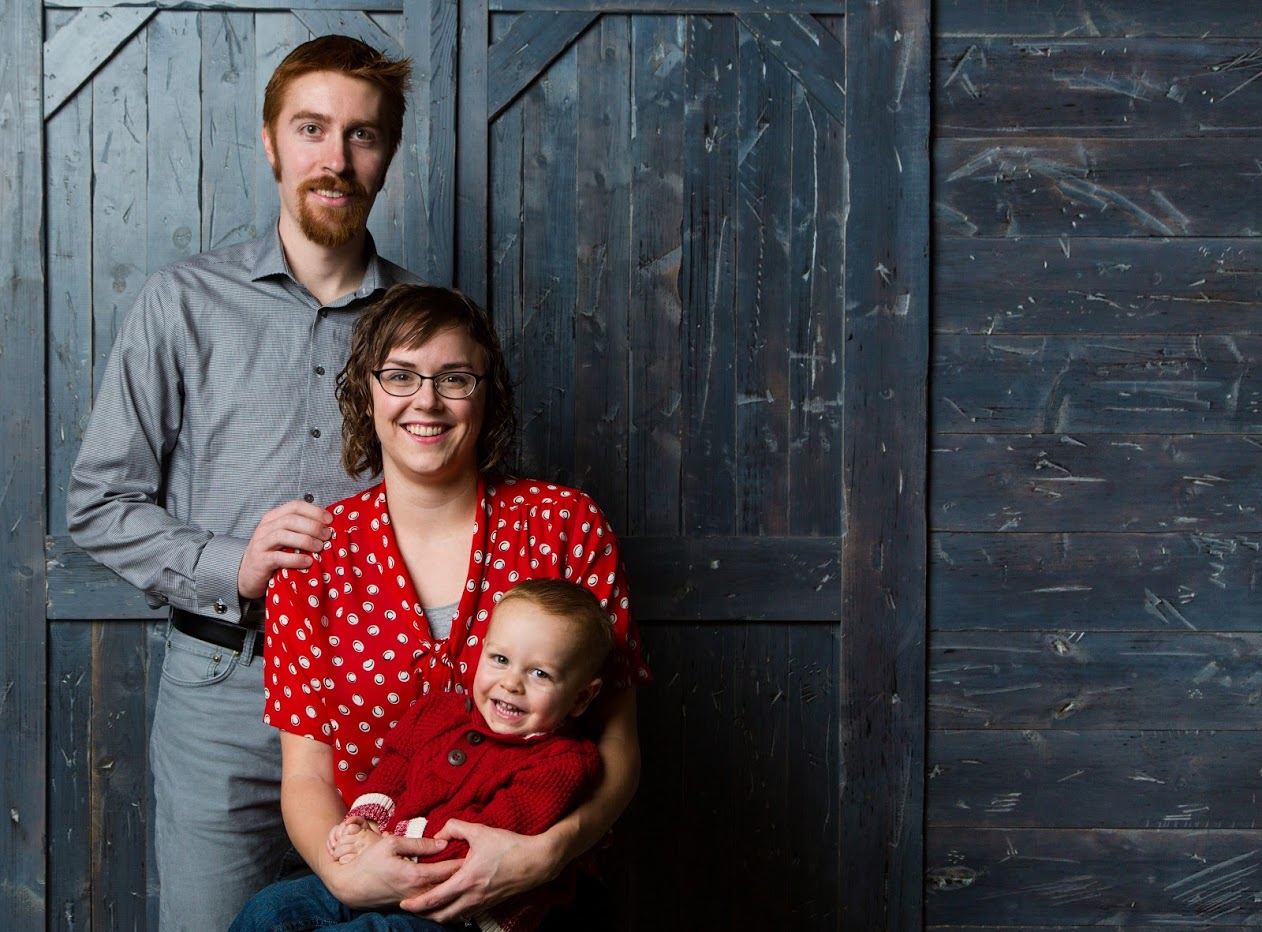
\includegraphics[width=0.7\linewidth]{./Family_photo}
\label{fig:Family_photo}
%TODO update photo
\end{figure}

\end{frame}

\begin{frame}{education}
\begin{itemize}
\item B.S. in Mechanical Engineering from Brigham Young University
\begin{itemize}
\item Worked with ATK to develop tab-less gripping system for tensile testing composite tow specimens
\item Needed to align the specimen, as well as grip it without causing a stress concentration
\end{itemize}
\item M.S. and Ph.D. from School of Aeronautics and Astronautics at Purdue University
\begin{itemize}
\item Worked with Boeing to simulate mold flows
\item First ever mold simulation with anisotropic viscosity
\end{itemize}
\end{itemize}
\end{frame}

\begin{frame}{research}
\begin{figure}
\centering
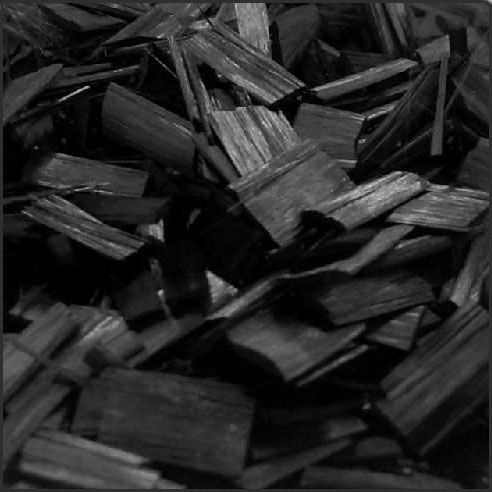
\includegraphics[width=0.6\linewidth]{./Formosa_Chopped_Carbon_Fiber_CSc_bw}
\label{fig:Formosa_Chopped_Carbon_Fiber_CSc_bw}
\end{figure}

\end{frame}

\begin{frame}{research}
\begin{figure}
\centering
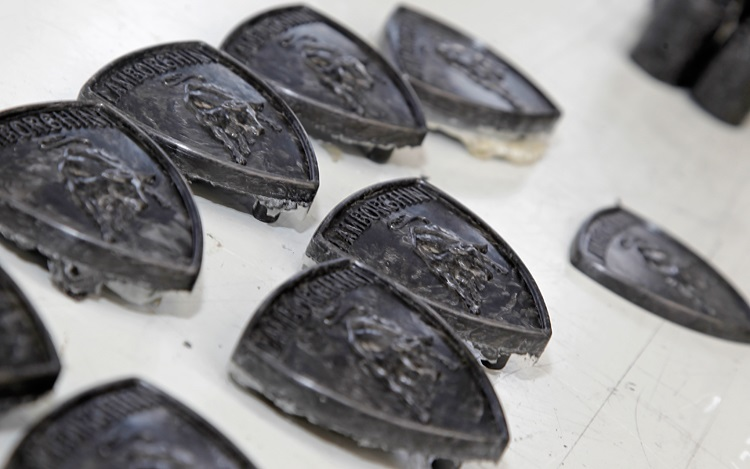
\includegraphics[width=0.8\linewidth]{./lamborghini-chopped-fiber-badges-rough}
\label{fig:lamborghini-chopped-fiber-badges-rough}
\end{figure}

\end{frame}

\begin{frame}{research}
\begin{itemize}
\item No simulation is currently able to predict fiber orientation from these processes
\item Part of the challenge is that we only have information from initial state and final state
\item I want to quantify intermediate stages using a transparent mold
\end{itemize}
\end{frame}

\begin{frame}{research}
\begin{columns}
	\begin{column}{0.45\textwidth}
		\begin{figure}
		\centering
		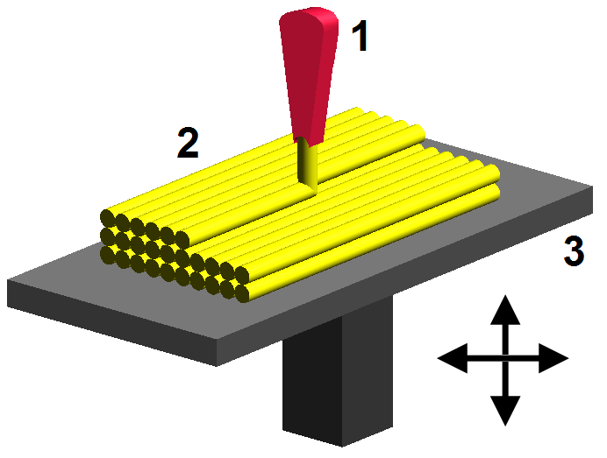
\includegraphics[width=0.9\columnwidth]{3D-printing}
		\label{fig:3D-printing}
		\end{figure}
	\end{column}
	\begin{column}{0.45\textwidth}
		\begin{itemize}
			\item Composites are being used in 3D printing now
			\item Printing patterns are optimized for isotropic materials
			\item Sometimes composites hurt more than they help when not utilized properly
		\end{itemize}
	\end{column}
\end{columns}
\end{frame}

\begin{frame}{introductions}
\begin{itemize}
\item Name
\item Student status (Undergrad, Masters, Ph.D)
\item Full time or part time student?
\item One interesting thing to remember you by
\end{itemize}
\end{frame}

\section{Syllabus and Schedule}

\begin{frame}{course textbook}
  \begin{itemize}
  \item Printed notes from Dr. Bert L. Smith and Dr. Walter J. Horn
  \item Will be available starting Thursday, bring \$25 cash or check to AE offices to pick up your copy
  \item Homework will be given in handouts
  \item Textbook is an assimilation of knowledge from many sources, provides excellent practical applications of fracture mechanics
  \item Supplemental textbooks are listed in the syllabus and in the text for further study
  \end{itemize}
\end{frame}

\begin{frame}{office hours}
  \begin{itemize}
  \item I will e-mail everyone in the course a Doodle link we can use to find the optimal office hours
  \item Let me know if you do not receive the e-mail, you may need to update your information in Blackboard
  \item Take advantage of office hours, this is time that I have already set aside for you
  \item If the regular office hours do not work for your schedule, send me an e-mail and we can work out a time to meet
  \item While in person visits are often the most helpful, I will always try to answer questions as best as I can via e-mail
  \end{itemize}
\end{frame}

\begin{frame}{tentative course outline}
\begin{itemize}
\item Section 1 - fracture mechanics
\begin{itemize}
	\item Stress intensity (19-26 Jan)
	\item Plastic zone (28 Jan - 4 Feb)
	\item Fracture toughness (9-16 Feb)
	\item Residual strength (18-25 Feb)
	\item Exam 1 (8 March)
\end{itemize}
\end{itemize}
\end{frame}

\begin{frame}{tentative course outline}
	\begin{itemize}
		\item Section 2 - fatigue
		\begin{itemize}
			\item Crack growth (10-24 Mar)
			\item Crack propagation (29 Mar - 5 Apr)
			\item Exam 2 (14 April)
		\end{itemize}
	\end{itemize}
\end{frame}

\begin{frame}{tentative course outline}
	\begin{itemize}
		\item Section 3 - damage tolerance
		\begin{itemize}
			\item Damage tolerance (7-21 Apr)
			\item Test methods (26-28 Apr)
			\item Finite elements (3-5 May)
			\item Non-Destructive Testing (time permitting)
			\item Final project (due 5 May)
		\end{itemize}
	\end{itemize}
\end{frame}

\begin{frame}{grades}
\begin{columns}
\column{0.5\textwidth}
\begin{itemize}
\item Grade breakdown
	\begin{itemize}
	\item Homework \dotfill 15\%
	\item Exam 1 \dotfill 30\%
	\item Exam 2 \dotfill 30\%
	\item Final Project \dotfill 25\%
	\end{itemize}
\item Follow a traditional grading scale
\end{itemize}
\column{0.5\textwidth}
\end{columns}
\begin{table}[H]
\resizebox{\textwidth}{!}{ %
\begin{tabular}{cccccccccccc}
 A & A- & B+ & B & B- & C+ & C & C- & D+ & D & D- & F \\ 
 93-100 & 90-93 & 87-90 & 83-87 & 80-83 & 77-80 & 73-77 & 70-73 & 67-70 & 63-67 & 60-63 & 0-60 
\end{tabular} %
}
\end{table}
\end{frame}

\begin{frame}{final project}
	\begin{itemize}
		\item Perform residual strength, fatigue and damage tolerance analysis on a real part
		\item Examples: car axle, fuselage panel, wing panel, landing gear, bike pedal
		\item Individual project
		\item More discussion after Exam 1
	\end{itemize}
\end{frame}

\begin{frame}{class expectations}
\begin{itemize}
\item Consider the cost (to you or others) of your being in class
\item I ask that you refrain from distracting behaviors during class
\item When you have something more important than class to take care of, please take care of it outside of class
\end{itemize}
\end{frame}

\section{Course Overview}

\begin{frame}{damage}
	\begin{itemize}
		\item In linear elasticity, we generally consider materials in their pristine state
		\item Realities of manufacturing, cyclic loads, and unforeseen loads result in a material which is something other than pristine
		\item In this course we will develop methods for predicting the strength of a material with some damage (residual strength)
		\item We will learn to predict the rate at which damage will grow (fatigue)
	\end{itemize}
\end{frame}

\begin{frame}{damage tolerance}
	\begin{itemize}
		\item There are many ways to address the problem of damage in a material
		\begin{enumerate}
			\item Infinite-life design
			\item Safe-life design
			\item Damage tolerant design
		\end{enumerate}
		\item To ensure damage tolerant design, we must ensure that crack growth is always stable
		\item Another important concept of damage tolerant design is to include multiple load paths, so failure in one part does not cause critical failure of the whole structure
	\end{itemize}
\end{frame}

\begin{frame}{damage tolerance}
\begin{figure}
\centering
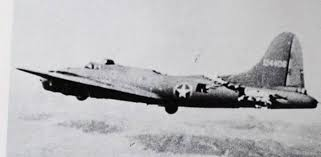
\includegraphics[width=0.7\linewidth]{B17}
\label{fig:B17}
\end{figure}
\end{frame}

\begin{frame}{damage tolerance}
	\begin{figure}
		\centering
		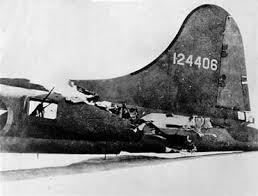
\includegraphics[width=0.7\linewidth]{B17a}
		\label{fig:B17a }
	\end{figure}
\end{frame}

\begin{frame}{damage tolerance}
	\begin{itemize}
		\item A B-17 collided with a Germain plane during WWII
		\item In spite of the damage, the B-17 was able to fly 90 minutes and land safely
	\end{itemize}
\end{frame}

\begin{frame}{damage tolerance}	
\begin{figure}
\centering
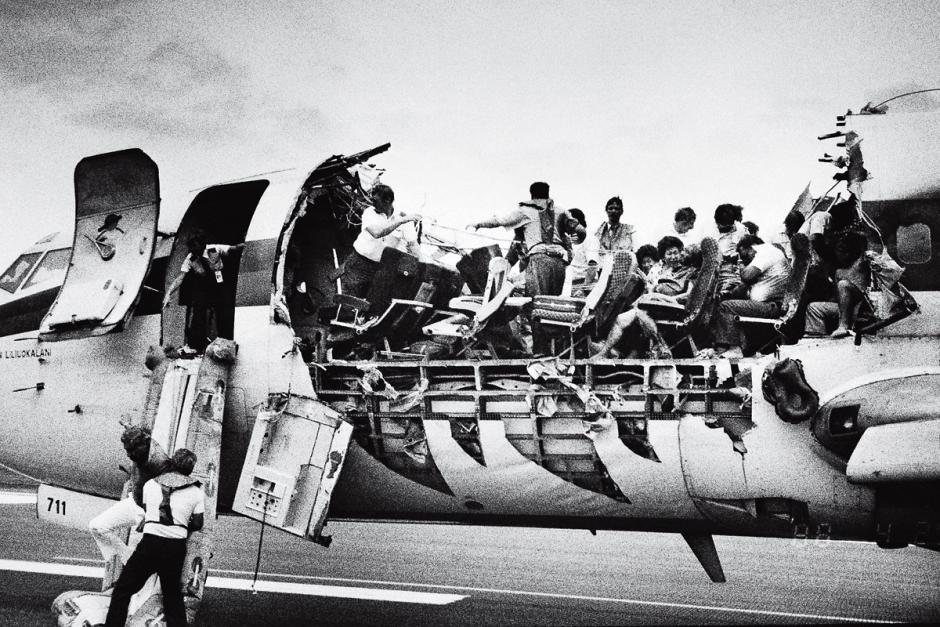
\includegraphics[width=0.7\linewidth]{737}
\label{fig:737}
\end{figure}
\end{frame}

\begin{frame}{damage tolerance}
	\begin{itemize}
		\item An example of multiple damaged sites occurred on a Boeing 737 in 1988
		\item Damage around multiple rivet holes connected and a full piece of the fuselage was blown off
		\item The plane was able to land safely
		\item This particular instance led to the study of "Multiple Site Damage"
	\end{itemize}
\end{frame}

\section{Fracture Mechanics}

\begin{frame}{fracture mechanics}
	\begin{itemize}
		\item \emph{Linear Elastic Fracture Mechanics} is the study of the propagation of cracks in materials
		\item There are some corrections we add to account for plasticity
		\item In this course we will not follow the full mathematical development of fracture mechanics (there is a separate course dedicated to that)
		\item Instead we will take some results and apply them
	\end{itemize}
\end{frame}

\begin{frame}{fracture mechanics}
	\begin{itemize}
		\item In fracture mechanics we consider three different modes
		\item Mode I is known as the "opening mode"
		\item Mode II is known as the "sliding mode"
		\item Mode III is known as the "tearing mode"
	\end{itemize}
\end{frame}

\begin{frame}{fracture mechanics}
	\begin{figure}
	\def\svgwidth{\linewidth}
	\input{Fracture_modes_v2.pdf_tex}
	\end{figure}
\end{frame}

\section{Stress Intensity}

\begin{frame}{stress intensity}
	\begin{itemize}
		\item A key finding from Linear Elastic Fracture Mechanics (LEFM) is known as the \emph{Stress Intensity Factor}
		\item The stress intensity factor is often written in this form
		\begin{equation}
		K = \sigma\sqrt{\pi a} \beta
		\end{equation}
		\item Where $K$ is the stress intensity factor, $\sigma$ is the applied stress, $a$ is the crack length, and $\beta$ is a dimensionless parameter depending on geometry
		\item Be careful that although the notation is similar, the \emph{Stress Intensity Factor} is different from the \emph{Stress Concentration Factor} from strength of materials
		\item We are usually most concerned with Mode I, but there will be a unique stress intensity factor for each mode, we label these $K_I$, $K_{II}$, and $K_{III}$
		\item If no subscript is given, assume Mode I
	\end{itemize}
\end{frame}

\begin{frame}{stress intensity}
	\begin{itemize}
		\item For brittle materials (where "linear" fracture mechanics assumptions hold true) we can find the full stress field near the crack in terms of the stress intensity factor
		\begin{align}
		\begin{split}
		\sigma_x &= \frac{K_I}{\sqrt{2\pi r}} \cos \frac{\theta}{2} \left(1-\sin \frac{\theta}{2}\sin \frac{3\theta}{2}\right)\\
		\sigma_y &= \frac{K_I}{\sqrt{2\pi r}} \cos \frac{\theta}{2} \left(1+\sin \frac{\theta}{2}\sin \frac{3\theta}{2}\right)\\
		\tau_{xy} &= \frac{K_I}{\sqrt{2\pi r}} \sin \frac{\theta}{2} \cos \frac{\theta}{2}\cos \frac{3\theta}{2}
		\end{split}
		\end{align}
	\end{itemize}
\end{frame}

\begin{frame}{stress intensity}
	\begin{itemize}
		\item Similarly for Mode II we find
		\begin{align}
		\begin{split}
		\sigma_x &= \frac{-K_{II}}{\sqrt{2\pi r}} \sin \frac{\theta}{2} \left(2+\cos \frac{\theta}{2}\cos \frac{3\theta}{2}\right)\\
		\sigma_y &= \frac{K_{II}}{\sqrt{2\pi r}} \sin \frac{\theta}{2} \cos \frac{\theta}{2}\cos \frac{3\theta}{2}\\
		\tau_{xy} &= \frac{K_{II}}{\sqrt{2\pi r}} \cos \frac{\theta}{2} \left(1-\sin \frac{\theta}{2}\sin \frac{3\theta}{2}\right)
		\end{split}
		\end{align}
	\end{itemize}
\end{frame}

\begin{frame}{stress intensity}
	\begin{itemize}
		\item And for Mode III
		\begin{align}
		\begin{split}
		\tau_{xz} &= \frac{-K_{III}}{\sqrt{2\pi r}} \sin \frac{\theta}{2} \\
		\tau_{yz} &= \frac{K_{III}}{\sqrt{2\pi r}} \cos \frac{\theta}{2} 
		\end{split}
		\end{align}
	\end{itemize}
\end{frame}

\section{Plotting}

\begin{frame}{plotting}
	\begin{itemize}
		\item Plotting is an important part of graduate work, and this course
		\item There are many software programs which can generate good scientific plots
		\begin{itemize}
			\item Microsoft Excel
			\item MATLAB
			\item Maple
			\item Mathematica
			\item Python
			\item R
			\item Plot.ly
		\end{itemize}
		\item You are welcome to use whatever software you desire, I will use Python for a quick demonstration
	\end{itemize}
\end{frame}

\begin{frame}{plotting}
	\begin{itemize}
		\item To make a good scientific plot, we must first decide what we are plotting, and which plot style will best illustrate our data
		\item Let us consider the Mode I stresses near a crack tip
		\begin{align*}
		\sigma_x &= \frac{K_I}{\sqrt{2\pi r}} \cos \frac{\theta}{2} \left(1-\sin \frac{\theta}{2}\sin \frac{3\theta}{2}\right)\\
		\sigma_y &= \frac{K_I}{\sqrt{2\pi r}} \cos \frac{\theta}{2} \left(1+\sin \frac{\theta}{2}\sin \frac{3\theta}{2}\right)\\
		\tau_{xy} &= \frac{K_I}{\sqrt{2\pi r}} \sin \frac{\theta}{2} \cos \frac{\theta}{2}\cos \frac{3\theta}{2}
		\end{align*}
		\item One interesting plot could be to examine stress magnitudes along the crack propagation direction as we get farther away from the crack
		\item In this case we would have $\theta = 0$.
		\item Since $\theta$ is a constant, it is not ideal to use a polar plot, instead we will use a standard rectangular plot
	\end{itemize}
\end{frame}

\begin{frame}{plotting}
	\begin{itemize}
		\item Since we are looking at stresses near the crack tip, it is convenient to normalize the distance by the crack length
		\item If substitute for $\theta$ and $K_I$ we have
		\begin{align*}
		\sigma_x &= \frac{\sigma\sqrt{\pi a} \beta}{\sqrt{2\pi r}} \\
		\sigma_y &= \frac{\sigma\sqrt{\pi a} \beta}{\sqrt{2\pi r}} \\
		\tau_{xy} &= 0
		\end{align*}
		\item Since $\sigma_x$ and $\sigma_y$ are identical for this case, we consider only one, and normalize by the applied stress. After simplification
		\begin{equation*}
		\frac{\sigma_x}{\sigma\beta} = \frac{1}{\sqrt{2}} \frac{1}{\sqrt{(r/a)}}
		\end{equation*}
	\end{itemize}
\end{frame}

\begin{frame}{plotting}
	\begin{figure}
	\centering
	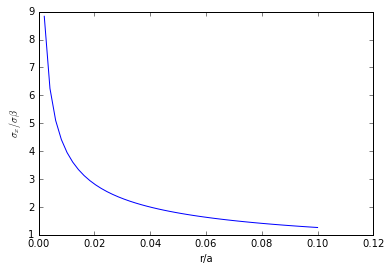
\includegraphics[width=0.7\linewidth]{sigmax_vs_ra}
	\caption{$\sigma_x$ for a Mode I crack plotted vs. normalized distance from crack tip, $r/a$.}
	\label{fig:sigmax_vs_ra}
	\end{figure}
\end{frame}

\begin{frame}{plotting}
	\begin{itemize}
		\item Since we found $\sigma_x = \sigma_y$ for $\theta=0$, we decide it might be better to look at a polar plot using $\theta$ as a variable
		\item To make a polar plot in this style, we need a function such that $r = f(\theta)$
		\item To do this we consider a constant stress value, we will solve for and plot the distance, $r$ at which the stress is equal to the same constant value for each of the three stress terms
		\begin{align*}
		\sigma_x = C &= \frac{K_I}{\sqrt{2\pi r}} \cos \frac{\theta}{2} \left(1-\sin \frac{\theta}{2}\sin \frac{3\theta}{2}\right)\\
		\sigma_y = C &= \frac{K_I}{\sqrt{2\pi r}} \cos \frac{\theta}{2} \left(1+\sin \frac{\theta}{2}\sin \frac{3\theta}{2}\right)\\
		\tau_{xy} = C &= \frac{K_I}{\sqrt{2\pi r}} \sin \frac{\theta}{2} \cos \frac{\theta}{2}\cos \frac{3\theta}{2}
		\end{align*}
	\end{itemize}
\end{frame}

\begin{frame}{plotting}
	\begin{itemize}
		\item After solving for $r$ we find
		\begin{align*}
		r &= \frac{K_I^2}{2 C^2 \pi} \cos^2 \frac{\theta}{2} \left(1-\sin \frac{\theta}{2}\sin \frac{3\theta}{2}\right)^2\\
		r &= \frac{K_I^2}{2 C^2 \pi} \cos^2 \frac{\theta}{2} \left(1+\sin \frac{\theta}{2}\sin \frac{3\theta}{2}\right)^2\\
		r &= \frac{K_I^2}{2 C^2 \pi} \sin^2 \frac{\theta}{2} \cos^2 \frac{\theta}{2}\cos^2 \frac{3\theta}{2}
		\end{align*}
	\end{itemize}
\end{frame}

\begin{frame}{plotting}
	\begin{figure}
	\centering
	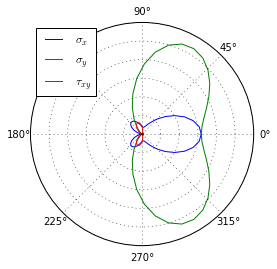
\includegraphics[width=0.7\linewidth]{polar_plot}
	\caption{Polar plot for constant stress contours near the crack tip for Mode I}
	\label{fig:polar_plot}
	\end{figure}
\end{frame}
\end{document}
